\documentclass{article}

\usepackage{graphicx}   %package for inserting graphs

\usepackage{geometry}
\geometry{
a4paper,
total={210mm,297mm},
left=20mm,
right=20mm,
top=20mm,
bottom=20mm,
}

\usepackage{graphicx}


\begin{document}

\title{Writing with \LaTeX{} in Stata Do-file Editor}
\author{E. F. Haghish}

\maketitle

\begin{abstract}
\textbf{MarkDoc} not only supports writing text using \textbf{Markdown Syntax} 
but also allows writing and styling text using \textbf{HTML} and \LaTeX{}. 
These new features will appeal only to professional users (\textit{Wierdos})
and the majority of the users will enjoy writing with Markdown. In this 
short turorial I will demonstrate how to weave a document in MarkDoc using 
\LaTeX{}. 
\end{abstract}

\section{Introduction}
There is a new feature in MarkDoc that allows you to weave your document
Using \LaTeX{}. This might only be interesting to some of you. 

Hey look, it's math.
\begin{equation}
\label{simple_equation}
\alpha = \sqrt{ \beta }
\end{equation}

\subsection{Adding Stata output}
Below I will add some Stata commands and outputs.

\begin{verbatim}
      
      

     1 . sysuse auto, clear      
      (1978 Automobile Data)
      

     2 . describe
      
      Contains data from C:\Program Files (x86)\Stata12\ado\base/a/auto.dta
        obs:            74                          1978 Automobile Data
       vars:            12                          13 Apr 2011 17:45
       size:         3,182                          (_dta has notes)
      --------------------------------------------------------------------------------
                    storage  display     value
      variable name   type   format      label      variable label
      --------------------------------------------------------------------------------
      make            str18  %-18s                  Make and Model
      price           int    %8.0gc                 Price
      mpg             int    %8.0g                  Mileage (mpg)
      rep78           int    %8.0g                  Repair Record 1978
      headroom        float  %6.1f                  Headroom (in.)
      trunk           int    %8.0g                  Trunk space (cu. ft.)
      weight          int    %8.0gc                 Weight (lbs.)
      length          int    %8.0g                  Length (in.)
      turn            int    %8.0g                  Turn Circle (ft.)
      displacement    int    %8.0g                  Displacement (cu. in.)
      gear_ratio      float  %6.2f                  Gear Ratio
      foreign         byte   %8.0g       origin     Car type
      --------------------------------------------------------------------------------
      Sorted by:  foreign
      

     3 . list in 1/3
      
           +---------------------------------------------------------------+
        1. | make        | price | mpg | rep78 | headroom | trunk | weight |
           | AMC Concord | 4,099 |  22 |     3 |      2.5 |    11 |  2,930 |
           |---------------------+-------------+---------------------------|
           |  length   |  turn   |  displa~t   |  gear_r~o   |   foreign   |
           |     186   |    40   |       121   |      3.58   |  Domestic   |
           +---------------------------------------------------------------+
      
           +---------------------------------------------------------------+
        2. | make        | price | mpg | rep78 | headroom | trunk | weight |
           | AMC Pacer   | 4,749 |  17 |     3 |      3.0 |    11 |  3,350 |
           |---------------------+-------------+---------------------------|
           |  length   |  turn   |  displa~t   |  gear_r~o   |   foreign   |
           |     173   |    40   |       258   |      2.53   |  Domestic   |
           +---------------------------------------------------------------+
      
           +---------------------------------------------------------------+
        3. | make        | price | mpg | rep78 | headroom | trunk | weight |
           | AMC Spirit  | 3,799 |  22 |     . |      3.0 |    12 |  2,640 |
           |---------------------+-------------+---------------------------|
           |  length   |  turn   |  displa~t   |  gear_r~o   |   foreign   |
           |     168   |    35   |       121   |      3.08   |  Domestic   |
           +---------------------------------------------------------------+
      

     4 . hist price
      (bin=8, start=3291, width=1576.875)
      
      

     5 . graph export graph.png, width(400) replace
      (note: file graph.png not found)
      (file graph.png written in PNG format)
      
      


\end{verbatim}



\begin{figure}[htbp]
\centering
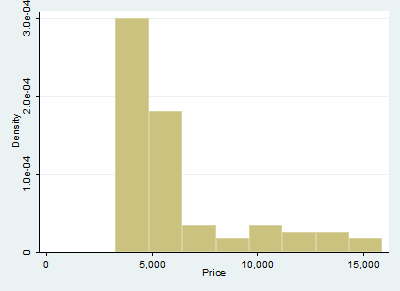
\includegraphics{graph.png}
\caption{This graph shows the histogram of the price variable}
\end{figure}



\section{Regression}
Let's end this do-file with a regression analysis.

\begin{verbatim}
      
      

     6 . regress price mpg
      
            Source |       SS       df       MS              Number of obs =      74
      -------------+------------------------------           F(  1,    72) =   20.26
             Model |   139449474     1   139449474           Prob > F      =  0.0000
          Residual |   495615923    72  6883554.48           R-squared     =  0.2196
      -------------+------------------------------           Adj R-squared =  0.2087
             Total |   635065396    73  8699525.97           Root MSE      =  2623.7
      
      ------------------------------------------------------------------------------
             price |      Coef.   Std. Err.      t    P>|t|     [95% Conf. Interval]
      -------------+----------------------------------------------------------------
               mpg |  -238.8943   53.07669    -4.50   0.000    -344.7008   -133.0879
             _cons |   11253.06   1170.813     9.61   0.000     8919.088    13587.03
      ------------------------------------------------------------------------------
      
      


\end{verbatim}

\section{Conclusion}
Writing a document with \LaTeX{} in \textbf{MarkDoc} is so natural and 
does not require additional options or commands. \textbf{MarkDoc} 
automatically recognizes that you are writing with \LaTeX{}. All that 
you need to do is to \textbf{export a tex file} from the options. Also 
remember not to mix HTML, \LaTeX{}, and Markdown in a single document. 
Make your mind what markup language you want to use for weaving your 
document. 

\end{document}
      
      
      
      





